\section{Echo State Network}
\label{sc:esn}
\subsection{Überblick}
Um die (Leistungs)Probleme der \textsc{RNN} zu umgehen, wurden als mögliche Lösung die \textsc{Echo State Networks} von H. Jäger vorgeschlagen \cite{jaeger2010}. Etwa zeitgleich wurde von W. Maas das Modell der \textit{Liquid State Machines} vorgeschlagen. In diesem Modell steht der biologische Hintergrund im Fokus, doch sind die Ergebnisse denen der \textsc{Echo State Networks} sehr ähnlich \citep{Maass2011}. 

\subsection{Aufbau}
\label{sec:esn_structure}
Ein \textsc{ESN} ist eine Spezialform eines \textsc{RNN}s. Hierbei wird eine auf dem ersten Blick eigenartige Entscheidung getroffen: Während des gesamten Trainingsvorganges werden die Verbindungen der einzelnen Einheiten größtenteils nicht verändert. Es wird versucht durch das \textit{Echo} der vorherigen Signale, welche noch im Netzwerk gespeichert sind, diese Signale zu rekonstruieren - hieraus ergibt sich auch der Name \cite{lukoseviciusa2009}. Im Folgenden wird der Aufbau und anschließend die Funktionsweise eines solchen Netzwerkes nach \citep{jaeger2007} beschrieben.\\

Allgemein bildet das Netzwerk $S$ ein zeitliches Signal $\vec{u}(n) \in \mathbb{R}^{N_u}$  auf eine zeitlich variable Ausgabe $\vec{y}(n) \in \mathbb{R}^{N_y}$ für die Zeiten $n=1, ..., T$ ab. Zudem besitzt das System ein sogenanntes \textsc{Reservoir} aus $N$ nicht-linearen Einheiten. Der innere Zustand des Netzwerkes wird durch diese Einheiten beschrieben und als $s(n) \in \mathbb{R}^{N}$ bezeichnet.\\
Die Verbindungen der inneren Einheiten untereinander werden durch die Gewichtsmatrix $\mathbf{W} \in \mathbb{R}^{N \times N}$ beschrieben. Das Eingangssignal wird zusammen mit einem \textit{Bias} $b_{in} \in \mathbb{R}$ durch die Matrix $\mathbf{W_{in}} \in \mathbb{R}^{N \times (N_u+1)}$ auf die inneren Einheiten weitergeleitet.\\

Die zeitliche Entwicklung der inneren Zustände berechnet sich nach der Vorschrift
\begin{align}
\label{eq:esn_stateeq}
\vec{s}(n) = (1 - \alpha) \cdot \vec{x}(n-1)  + \alpha \cdot f_{in}\left( \mathbf{W_{in}} [b_{in}; \vec{u}(n)] + \mathbf{W} \vec{x}(n-1) \right),
\end{align}
wobei $f_{in}$ eine beliebige (meistens \textit{sigmoid}-förmige) Transferfunktion ist, und $[\cdot\,;\,\cdot]$ das vertikale Aneinanderfügen von Vektoren beziehungsweise Matrizen bezeichnet. Für diese Zustandsgleichung wurde das Modell eines \textit{Leaky Integrator Neurons} genutzt, wobei $\alpha \in (0,1]$ die Verlustrate beschreibt. Für $\alpha=1$ ergibt sich als Spezialfall ein gewöhnliches Neuron
\begin{align}
\vec{s}(n) = f_{in}\left( \mathbf{W_{in}} [b_{in}; \vec{u}(n)] + \mathbf{W} \vec{x}(n-1) \right).
\end{align}

Da für manche Anwendungsfälle auch eine direkte Rückkopplung wünschenswert ist, kann das System noch um eine Ausgabe-Rückkopplung erweitert werden. Diese verbindet die Ausgabe erneut mit den inneren Einheiten durch die Matrix $\mathbf{W_{fb}} \in \mathbb{R}^{N \times N_y}$.
Somit ergibt sich 
\begin{align}
\label{eq:esn_stateeq_feedback}
\vec{s}(n) = (1 - \alpha) \cdot \vec{x}(n-1)  \alpha \cdot f_{in}\left( \mathbf{W_{in}} [b_{in}; \vec{u}(n)] + \mathbf{W} \vec{x}(n-1) + \mathbf{W_{fb}} \vec{y}(n) \right)
\end{align}
als Zustandsgleichung. In Abbildung \ref{fig:esn_structure} ist der vollständige Struktur eines \textsc{ESN}s mit den Matrizen $\mathbf{W_{in}}, \mathbf{W}$ und $\mathbf{W_{out}}$ dargestellt.

\begin{figure}[H]
    \centering
    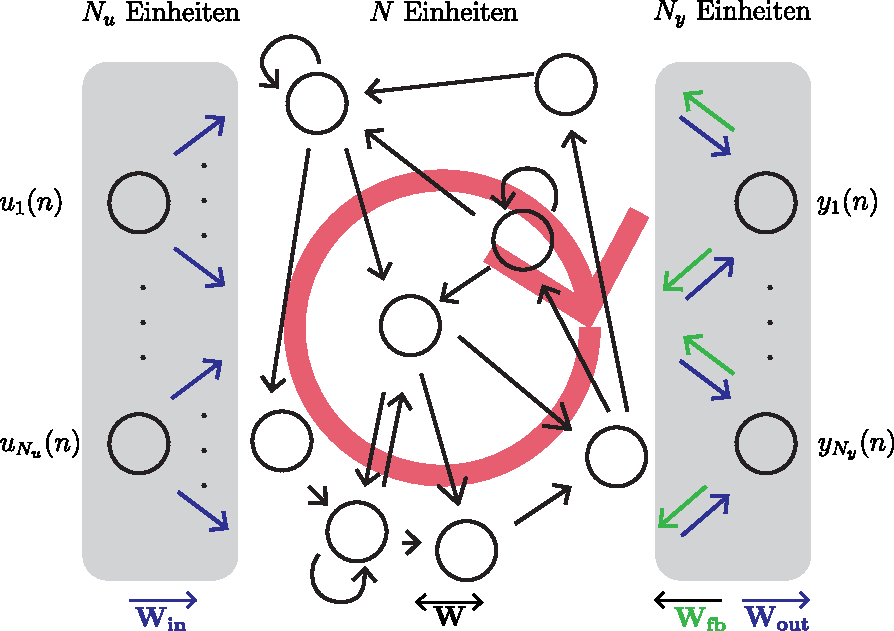
\includegraphics[width = 0.7 \textwidth]{figures/illustrations/esn_structure.pdf}
    \caption{Schematische Darstellung eines \textsc{ESN}. Von links nach rechts durchläuft das Eingangssignal $u(n)$ erst $N_u$ Eingangseinheiten, danach ein Reservoir mit $N$ Einheiten, bis schließlich die Ausgabe $y(n)$ mittels $N_y$ Ausgabeeinheiten gebildet wird. (nach \citep{jeagerTut2002, Ma2013}).}
    \label{fig:esn_structure}
\end{figure}


Anhand der inneren Zustände lassen sich nun noch die sogenannten erweiterten inneren Zustände $x(n) = [b_{out}; \vec{s}(n); \vec{u}(n)] \in \mathbb{R}^{1 + N_u + N}$ definieren, wobei $b_{out}$ ein \textit{Bias} für die Ausgabe darstellt. 

Aus diesen erweiterten inneren Zuständen kann nun die Ausgabe $\vec{y}(n)$ konstruiert werden. Dies kann entweder im Sinne einer Linearkombination durch die Ausgangsmatrix $\mathbf{W_{out}} \in \mathbb{R}^{(1 + N_u + N) \times N_y}$ oder durch andere nicht lineare Regressionsalgorithmen wie beispielsweise einer \textsc{Support Vector Machine (SVM)} durchgeführt werden. Im Folgenden wird nur der Fall einer Linearkombination betrachtet, da sich für die anderen Methoden ein analoges Verfahren ergibt.
In diesem Fall berechnet sich die Ausgabe mittels
\begin{align}
\vec{y}(n) = f_{out} \left( \mathbf{W_{out}} \vec{x}(n) = \mathbf{W_{out}} [b_{out}; \vec{s}(n); \vec{u}(n)] \right),
\end{align}
wobei $f_{out}$ die Transferfunktion der Ausgabe ist. Für diese kann in den meisten Fällen (so auch in dieser Arbeit) die Identität $f_{out}(x) = x$ genutzt werden.\\

Während die Matrix $\mathbf{W_{out}}$ durch den Trainingsvorgang bestimmt wird, werden die Matrizen $\mathbf{W_{in}}$ und $\mathbf{W}$ a priori generiert und festgelegt. Hierbei hat sich für das Generieren der Eingangsmatrix eine zufällige Anordnung von zufälligen Gleitkommazahlen zwischen $-0.5$ und $0.5$ als geschickt herausgestellt. Falls ein Feedback gewünscht ist, also Gleichung (\ref{eq:esn_stateeq_feedback}) genutzt wird, wird $\mathbf{W_{fb}}$ gleichartig konstruiert. Auf das Generieren der inneren Matrix $\mathbf{W}$ wird in Abschnitt \ref{sc:esn_theory} genauer eingegangen.

\subsection{Trainingsvorgang}
Nachdem der Aufbau des Netzwerkes beschrieben ist, ergibt sich nun die Frage, wie der Trainingsvorgang durchgeführt wird.

Hierfür wird für die Zeiten $n=0, ..., T_0$ das \textsc{ESN} mit dem Signal $\vec{u}(n)$ betrieben, wobei $T_0$ die \textit{transiente Zeit} beschreibt. Hierdurch soll das System aus seinem zufällig gewähltem Anfangszustand in einen charakteristischen Zustand übergehen. Anschließend wird das System für Zeiten $n < T$ weiter betrieben und die erweiterten Zustände $\vec{x}(n)$ als Spalten in der \textit{Zustandsmatrix} $\mathbf{X} \in \mathbb{R}^{(1 + N_u + N) \times T}$ gesammelt. Analog dazu werden die gewünschten Ausgaben $\vec{y}(n)$ nach dem Anwenden der Inversen $f^{-1}_{out}$ der Ausgabe-Transferfunktion $f_{out}$ auch als Spalten in der \textit{Ausgabematrix} $Y \in \mathbb{R}^{N_y \times T}$ gesammelt.
Nun wird eine Lösung der Gleichung
\begin{align}
\mathbf{Y} = \mathbf{W}_{out} \mathbf{X}
\end{align}
für $\mathbf{W}_{out}$ gesucht. Hierfür stehen mehrere Verfahren zur Verfügung, von denen zwei prominente erwähnt sein sollen.
Zum einen kann die Lösung durch eine \textit{Tikhonov Regularisierung} mittels der Regularisierung $\beta \cdot ||\vec{W}_{out, i}||^2$ der Gewichtsmatrix mit der Konstante $\beta$ erhalten werden. Hierbei steht $\vec{W}_{out, i}$ für die jeweils $i$-te Zeile der Gewichtsmatrix. Das Verfahren
\begin{align}
\label{eq:tikhonov}
\mathbf{W}_{out} = \mathbf{Y} \mathbf{X}^T \left(\mathbf{X} \mathbf{X}^T + \beta I \right)^{-1}
\end{align}
ist sehr leistungsstark, aber auch teilweise numerisch instabil. Bei geeigneter Wahl von $\beta$ können die besten Ergebnisse hinsichtlich der Genauigkeit der Vorsage erzielt werden \cite{lukoseviciusa2009}. Deshalb wird in dieser Arbeit auch nur dieses Lösungsverfahren verwendet. Die weiteren Lösungsansätze für das Gleichungssystem sind nur aus Gründen der Vollständigkeit angegeben.\\

Zum anderen kann zur Lösung die \textit{Moore-Penrose-Pseudoinverse} $\mathbf{X}'$ genutzt werden, sodass für die Ausgabematrix
\begin{align}
\label{eq:pseudo_inverse}
\mathbf{W}_{out} = \mathbf{Y} \mathbf{X}'
\end{align}
folgt. Dieses Verfahren ist zwar sehr rechenaufwendig aber dafür numerisch stabil \cite{lukoseviciusa2009, jaeger2012}. Nichts desto trotz, kann allerdings auf Grund des Fehlens einer Regularisierung leicht der Effekt des \textsc{Overfittings} auftreten. Auf Grund dessen wird es in dieser Arbeit nicht verwendet.\\

Um den Effekt des Overfittings bei der Verwendung der Psuedoinversen zu reduzieren, kann in der Zustandsgleichung (\ref{eq:esn_stateeq}) beziehungsweise (\ref{eq:esn_stateeq_feedback}) eine leichte normalverteilte Störung $\vec{\nu}(n)$ der Größenordnung $\num{1e-1}$ bis $\num{1e-5}$ addiert wird. Falls die \textit{Tikhonov Regularisierung} zur Lösung verwendet wird, erhöht die Verwendung der zufälligen Störung die Stabilität der Vorhersage des System. Dieser Ansatz beruht auf Empirie, da eine mathematische Begründung hierfür noch nicht vollständig gelungen ist \citep{jaeger2010, lukoseviciusa2009}. Anschaulich lässt sich das Vorgehen dadurch motivieren, dass hierdurch künstliche Datenpunkte in der nähe der vorhandenen Trainingsdaten emuliert werden, und somit eine größere Vielfalt an Daten während der Trainingsphase beobachtet wird.\\

Zusammenfassend ergibt sich somit der folgende Funktionsablauf für die Anwendung eines \textsc{ESN}:

\singlespacing
\begin{enumerate}
	\item Zufälliges Generieren der Matrizen $\mathbf{W}_{in}, \mathbf{W}_{fb}$ und Konstruktion der Matrix $\mathbf{W}$ 
	\item Einspeisen des Signals $u(n)$ und Konstruktion der Zustandsmatrix $\mathbf{X}$ und der Ausgabematrix $\mathbf{Y}$ 
	\item Berechnung der Ausgabematrix $\mathbf{W}_{out}$
	\item Einspeisen des Signals $u(n)$ für Vorhersagen des Signales $y(n)$ für $n > T$
\end{enumerate}
\onehalfspacing

Zusätzlich zu diesen Eigenschaften wird die Dynamik des Reservoirs auch von dessen Größe $N$ bestimmt. Es kann gezeigt werden, dass die Gedächtnisleistung eines Reservoirs stark von dieser abhängt. Somit ist es ratsam für Aufgaben, die eine lange Gedächtnisleistung benötigen, ein großes und für Aufgaben, die nur ein Kurzzeitgedächtnis benötigten, ein kleines Reservoir zu benutzen \citep{jeagerTut2002}.





\subsection{Theoretischer Hintergrund}
\label{sc:esn_theory}
Um die mathematischen Eigenschaften beschreiben zu können, sind zuerst zwei Definitionen nötig \cite{yildiz}.

\begin{definition}[Kompatibler Zustand]
Sei $S : X \times U \rightarrow X$ ein \textsc{ESN} mit der Zustandsgleichung $\vec{x}_{n+1} = F \left( \vec{x}_n, \vec{u}_{n+1} \right)$. Eine Folge von Zuständen $(\vec{x}_n)_n$ ist kompatibel mit der Eingangsfolge $(\vec{u}_n)_n$, wenn $\vec{x}_{n+1} = F\left( \vec{x}_n, \vec{u}_{n+1} \right), \forall n \leq 0$ erfüllt ist.
\end{definition}

\begin{definition}[Echo State Eigenschaft (ESP)]
Ein \textsc{ESN} $S : X \times U \rightarrow X$ besitzt die \textit{Echo State Eigenschaft} genau dann wenn eine Nullfolge $(\delta_n)_{n \geq 0}$ existiert, sodass für alle Zustandsfolgen $(\vec{x}_n)_n, (\vec{x}'_n)_n$ die kompatibel mit der Eingangsfolge $(\vec{u}_n)_n$ sind gilt, dass $\forall n \geq 0 ||x_n - x'_n|| < \delta_n$
\end{definition} 
Dies bedeutet, dass nachdem das Netzwerk lang genug betrieben worden ist, der Zustand nicht mehr von dem beliebig gewähltem Anfangszustand abhängt. Diese Eigenschaft ist notwendig, damit das \textsc{ESN} Vorhersagen treffen kann \cite{jeagerTut2002}.\\

Nun stellt sich die Frage, wann ein Netzwerk diese Eigenschaft besitzt. Es wird schnell klar, dass dies hauptsächlich durch die Gewichtsmatrix $\mathbf{W}$ bestimmt wird. Betrachtet man die Zustandsgleichung des Netzwerkes, so lässt sich auf Grund des \textit{Banachschen Fixpunktsatzes} erkennen, dass die \textit{ESP} für alle Eingänge $\vec{u}_n$ vorliegt, sobald $||\vec{x}_{n+1} - \vec{x}'_{n+1}|| < ||\vec{x}_n - \vec{x}'_n||$ für zwei kompatible Zustände $\vec{x}_n \neq \vec{x}'_n$ erfüllt ist \cite{jaeger2010}.
Hieraus ergibt sich, dass die \textit{ESP} vorliegt, wenn 
\begin{align}
\label{eq:theory_old_requirement}
|1-\alpha(1-\sigma_{max}(\mathbf{W}))| < 1
\end{align}
erfüllt ist, wobei $\sigma_{max}(\mathbf{W})$ der größte Singulärwert ist \cite{jaeger2007}.\\
Weitergehend ist bekannt, dass für Systeme bei denen der Spektralradius $\rho(\mathbf{W}) > 1$ ist diese Eigenschaft nicht vorliegen kann, sofern $\vec{u}_n = 0$ möglich ist \cite{jaeger2007, jaeger2010}.\\

Hieraus ergab sich lange Zeit die falsche Annahme, dass für Systeme mit $\rho(\mathbf{W}) < 1$ die Eigenschaft stets garantiert ist. Wie allerdings gezeigt werden konnte, ist dies nicht der Fall \citep{yildiz}. Stattdessen konnte gezeigt werden, dass eine hinreichende Bedingung durch
\begin{align}
\label{eq:theory_sufficient_requirement}
\rho(\alpha |\mathbf{W}|+(1-\alpha) \mathbf{I}) < 1
\end{align}
gegeben ist - wobei als Betrag der Matrix hier das elementweise Betragsnehmen gemeint ist. Diese Bedingung ist weniger einschränkend als Gleichung (\ref{eq:theory_old_requirement}) \cite{yildiz}.\\

Weitergehend hat sich in Experimenten gezeigt, dass eine dünnbesetze Gewichtsmatrix $\mathbf{W}$ zu reicheren Dynamiken innerhalb des Reservoirs führen kann \citep{jaeger2010}. Eine solche dünnbesetze Matrix bedeutet, dass nicht mehr jedes Neuron mit jedem anderen Neuron verbunden ist, sondern dass nur noch ein relativer Anteil $\epsilon$ dieser Verbindungen vorhanden ist. Da durch eine größere Anzahl an verschiedenen internen Dynamiken vielfältigere Funktionen besser approximiert werden können, kann die Vorhersagequalität durch einen Geringen $\epsilon$ Wert erhöht werden.\\

Darauf basierend kann nun eine Methode nach \cite{yildiz} angegeben werden, um die Gewichtsmatrix $\mathbf{W}$ zu konstruieren:

\singlespacing
\begin{enumerate}
	\item Generiere zufällige Matrix $\mathbf{W}$ mit $\mathbf{|W|} = \mathbf{W}$ bei der in jeder Zeile nur $\epsilon$ Einträge ungleich $0$ sind.
	\item Skaliere $\mathbf{W}$, sodass Gleichung (\ref{eq:theory_sufficient_requirement}) erfüllt ist.
	\item Wechsel zufällig das Vorzeichen von ungefähr der Hälfte aller Einträge.
\end{enumerate}
\onehalfspacing

Statt dieser Vorschrift wurde zuvor oftmals $\mathbf{W}$ zufällig generiert und anschließend nur $\rho(\mathbf{W})$ statt $\rho(|\mathbf{W}|)$ skaliert, was mit unter zu instabilen Systemen geführt hat. Da allerdings auch für Systeme mit einem Spektralradius $ > 1$ die \textit{ESP} beobachtet werden kann für nicht verschwindende Eingänge $\vec{u}_n$, ist es ratsam auch effektive Spektralradien jenseits $1$ auszuprobieren.